\section{Does a training profile choose a useful schedule?}
\label{sec:profile-results}
Table~\ref{tab:profile-results} evaluates the fixed 50-query rule from Section~\ref{sec:profile-protocol}. Across 140 configuration/split choices, it selects original order \ProfileOriginalChoices{} times, sorting \ProfileSortedChoices{} times and round-robin \ProfileRRChoices{} times. Each chosen order is then evaluated on its matching held-out stream. The choice counts make clear whether a gain comes from selecting a different schedule or simply recovering a consistently useful fixed one. When original order is selected, the result reuses the baseline stream: its zero difference and zero-width interval are identities, not a statistical equivalence test for a deployed frontend with overhead.

\begin{table}[htbp]\centering\small
\caption[Training-selected schedules on held-out queries]{BFS placement, 50 calibration queries and 200 held-out queries per split. O/S/R counts denote original/sorted/round-robin choices across ten splits. Differences from original order are means with paired 95\% intervals; the oracle gap is the mean excess over the best fixed order chosen retrospectively for each held-out split. Lower is better.}\label{tab:profile-results}
\resizebox{\textwidth}{!}{\begin{tabular}{lrrrr}
\toprule
Condition & Bytes & Choices O/S/R & vs original (\%) & Oracle gap (\%) \\
\midrule
Default (64 outstanding) & 512 & 0/0/10 & -14.58 [-14.64, -14.51] & 0.000 \\
Default (64 outstanding) & 128 & 10/0/0 & +0.00 [+0.00, +0.00] & 0.000 \\
16 outstanding & 512 & 0/0/10 & -33.08 [-33.21, -32.94] & 0.000 \\
16 outstanding & 128 & 0/0/10 & -10.61 [-10.68, -10.54] & 0.000 \\
32 outstanding & 512 & 0/0/10 & -21.86 [-21.95, -21.78] & 0.000 \\
32 outstanding & 128 & 10/0/0 & +0.00 [+0.00, +0.00] & 0.000 \\
128 outstanding & 512 & 0/0/10 & -14.58 [-14.64, -14.51] & 0.000 \\
128 outstanding & 128 & 10/0/0 & +0.00 [+0.00, +0.00] & 0.000 \\
Candidate batches of 2 & 512 & 0/0/10 & -7.77 [-7.79, -7.76] & 0.000 \\
Candidate batches of 2 & 128 & 0/0/10 & -1.48 [-1.51, -1.46] & 0.000 \\
Candidate batches of 8 & 512 & 0/0/10 & -15.55 [-15.60, -15.50] & 0.000 \\
Candidate batches of 8 & 128 & 0/0/10 & -2.48 [-2.52, -2.43] & 0.000 \\
Alternative address mapping & 512 & 10/0/0 & +0.00 [+0.00, +0.00] & 0.000 \\
Alternative address mapping & 128 & 0/10/0 & -0.34 [-0.36, -0.33] & 0.000 \\
\bottomrule
\end{tabular}
}
\end{table}

The training choice matches the retrospectively best fixed order in \ProfileOracleMatches{} of 140 held-out configuration/split cases. The largest mean and single-split oracle gaps are \ProfileMaxMeanRegret\% and \ProfileMaxSplitRegret\%, with \ProfileOriginalRegressions{} aggregate regressions relative to original order. Each configuration receives the same choice across all ten training splits. Profiling therefore recovers a consistently useful fixed order in this matrix; these data do not show a need for per-query adaptation.

This is an observed result on the evaluated workload, not a guarantee for future queries. The policy was motivated by previously inspected outcomes, and its evaluation remains exploratory. A different query distribution could favour another order. Original order is one of the candidates, not a mathematical protection against held-out regression.

Aggregate gains can also coexist with slower individual queries. Table~\ref{tab:profile-query} retains the slower-query fraction and empirical 95th-percentile service change for the selected path under every setting. Under the alternative mapper at 128 bytes, 20.5--28.0\% of individual queries are slower across the ten splits, and the 95th-percentile change ranges from a 0.68\% reduction to a 0.38\% increase despite the aggregate saving. Small batches at 128 bytes also contain individual regressions. These are descriptive checks of the same query records; they are not additional independent trials or a bound on production tail latency.

\begin{figure}[htbp]\centering
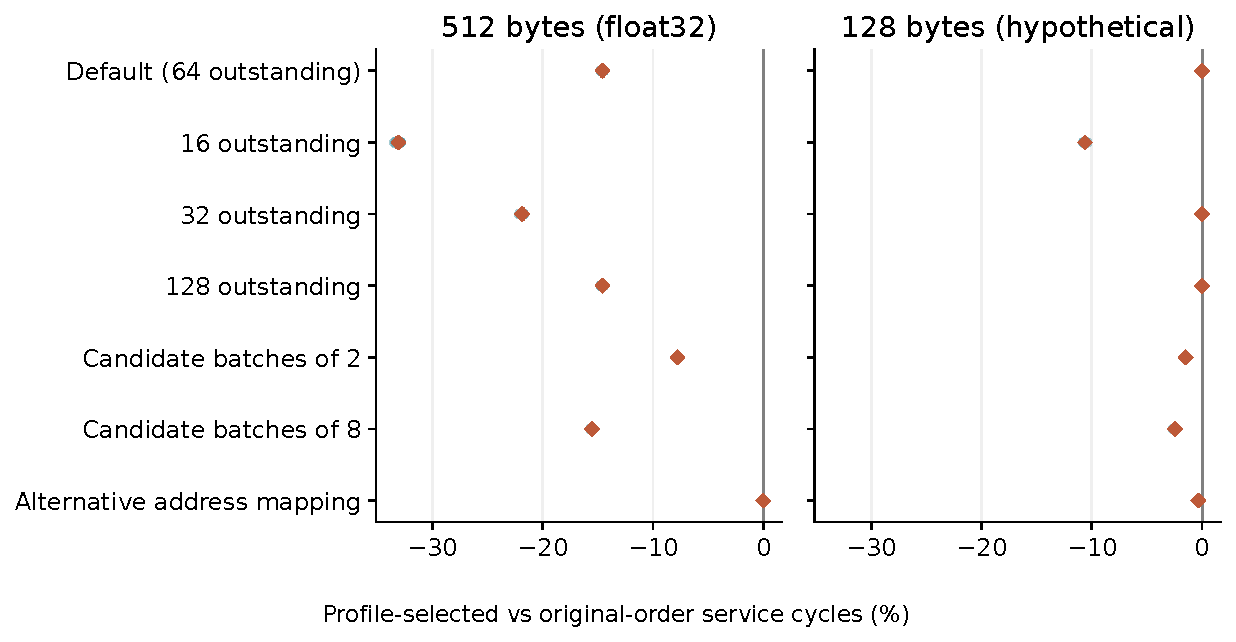
\includegraphics[width=\textwidth]{generated/profiled_fetch.pdf}
\caption[Held-out effect of the training-selected path]{Selected schedule versus original order under each matching configuration. Faint points show all ten split effects; diamonds and bars show means and paired 95\% intervals. Selection uses training cycles only. The footprint and one-setting-at-a-time restrictions are the same as in Figure~\ref{fig:scheduling-sensitivity}.}\label{fig:profiled-fetch}
\end{figure}

\subsection{Comparison with existing methods}
At default settings, Table~\ref{tab:profile-baselines} compares the selected BFS path with every fixed BFS schedule and the published placement routines under original-order bounded replay. The comparison to a fixed schedule is necessary: selecting round-robin does not improve on round-robin itself. Comparisons to RCM, Gorder and Porder change both placement and scheduling; they test the complete measured configurations. At 512 bytes, the selected path differs from Porder with original order by \ProfileVsPorderFloat\%; at the hypothetical 128-byte footprint, it uses original order and differs from Gorder by \ProfileVsGorderCompact\%. The proposal therefore complements the placement comparison without winning every baseline. These results do not establish that BFS plus profiling is optimal, or predict how a published placement would behave with the same selector.

\begin{table}[htbp]\centering\small
\caption[Profiled path versus measured baselines]{Default memory configuration and expansion boundaries. Mean paired cycle difference (\%) and 95\% interval across ten reference splits. Original, sorted and round-robin use BFS; RCM, Gorder and Porder use their respective placements and original order. The oracle is descriptive and uses held-out outcomes.}\label{tab:profile-baselines}
\begin{tabular}{lrr}
\toprule
Bytes & Comparator & Profiled path difference (\%) \\
\midrule
512 & Original & -14.58 [-14.64, -14.51] \\
512 & Sorted & -14.73 [-14.81, -14.66] \\
512 & Round-robin & +0.00 [+0.00, +0.00] \\
512 & Oracle & +0.00 [+0.00, +0.00] \\
512 & RCM & -14.44 [-14.53, -14.35] \\
512 & Gorder & -14.40 [-14.50, -14.31] \\
512 & Porder & -14.25 [-14.36, -14.14] \\
128 & Original & +0.00 [+0.00, +0.00] \\
128 & Sorted & -0.17 [-0.21, -0.12] \\
128 & Round-robin & -3.31 [-3.42, -3.20] \\
128 & Oracle & +0.00 [+0.00, +0.00] \\
128 & RCM & +0.47 [+0.38, +0.56] \\
128 & Gorder & +1.35 [+1.26, +1.44] \\
128 & Porder & +1.20 [+1.05, +1.35] \\
\bottomrule
\end{tabular}

\end{table}

The artifact also retains comparisons against every fixed order in every sensitivity condition in \texttt{results/profiled\_fetch\_summary.csv}. Published PIM systems are positioned by method and scope in Table~\ref{tab:related}; their end-to-end speedups cannot serve as numerical baselines for a trace-service percentage on different hardware and workloads.

\subsection{What the profile costs}
Calibration executes three 50-query streams per configuration, even though deployment uses only one schedule. Table~\ref{tab:profile-service} also gives absolute service for every setting: a larger percentage saving against a slower baseline does not establish that the whole configuration is faster. For example, the selected 512-byte path averages 41,316 service cycles per query at limit 16, compared with 34,008 at the default limit, despite its larger relative reduction. Appendix~\ref{app:profile-cost} reports that total service cost and the held-out saving per query separately. The experiment omits the cost of collecting a profile on the target, performing selection, storing the configuration key and executing the chosen order. A configuration with little or no service saving has correspondingly little room to recover those costs. Profiling is most relevant to a stable graph and workload that can reuse the choice; its application-level break-even point remains unmeasured.
